\documentclass{beamer}
\usetheme{metropolis}
\usepackage{latexsym}
\usepackage{amssymb}
\usepackage{amsbsy}
\usepackage{alltt}
\usepackage{tikz}
\usetikzlibrary{shapes}
\usetikzlibrary{shapes.symbols}
\usepackage{stmaryrd}
\usepackage{graphicx}

\newcommand{\imp}{\Rightarrow}
\newcommand{\etal}{\textit{et. al}}
\newcommand{\adhoc}{\textit{ad hoc}}
\newcommand{\ie}{\textit{i.e.}}
\newcommand{\etc}{\textit{etc}}
\newcommand{\eg}{\textit{e.g.}}
\newcommand{\kemph}[1]{\colorbox{orange}{#1}}
\newcommand{\gemph}[1]{\colorbox{green}{#1}}
\newcommand{\konst}[1]{\ensuremath{\mbox{\bf{#1}}}}
\newcommand{\nil}{\konst{[\,]}}
\newcommand{\cons}[2]{{#1}\boldsymbol{:}\boldsymbol{:}{#2}}
\newcommand{\hollamb}{\boldsymbol{\lambda}}
\newcommand{\kstar}[1]{\ensuremath{{#1}^{*}}}
\newcommand{\itelse}[3]{\mbox{$\mbox{\tt if}\ {#1}\ \mbox{\tt then}\ {#2}\
    \mbox{\tt else}\ {#3}$}}
\newcommand{\set}[1]{\{ {#1} \}}
\newcommand{\Lang}[1]{\ensuremath{{\cal L}({#1})}}
\newcommand{\LangTheta}[1]{\ensuremath{{\mathcal L}_{\theta}({#1})}}
\newcommand{\inbox}[1] {\begin{center}
                         \framebox{\parbox{0.984\textwidth}{#1}}
                         \end{center}}

% for backslashes in alltt environments
\newcommand{\bs}{\texttt{\symbol{92}}}

\begin{document}

% Title page

\author{Konrad Slind \\ Collins Aerospace}
\date{ITP 2021 \par June 30 2021}
\title{Specifying Message Formats \\ with Contiguity Types}
\maketitle

\begin{frame}\frametitle{Overview}

\begin{enumerate}
\item [$\blacktriangleright$] Data Formats and Self-Describing Messages
\item [$\blacktriangleright$] Contiguity Types
\item [$\blacktriangleright$] Applications
\item [$\blacktriangleright$] Extensions and Future Work
\end{enumerate}
\end{frame}


\begin{frame}\frametitle{Data Formats}

\begin{itemize}

\item [$\blacktriangleright$] A \gemph{Data Format} is a specification of how serialized data
  is laid out into a flat string (byte array).

\item [$\blacktriangleright$] Examples range from ISA descriptions, to network message
  formats, to file formats for document languages such as PDF, to all
  manner of ad hoc file formats cooked up so that people can share
  data on computers.

\item [$\blacktriangleright$] Very simple example:

\[
\begin{array}{l}
    \underbrace{\fbox{\quad Field 1\qquad}}_{\substack{\text{4 bytes} \\\ \text{int32}}}
    \underbrace{\fbox{Field 2}}_{\substack{\text{1 byte} \\\ \text{char}}}
    \underbrace{\fbox{\qquad Field 3 \qquad}}_{\substack{\text{8 bytes} \\\ \text{double}}}
  \end{array}
\]

\item [$\blacktriangleright$] The world is \gemph{filled to overflowing} with data formats

\end{itemize}
\end{frame}


\begin{frame}\frametitle{Data Description Languages}

\begin{itemize}

\item [$\blacktriangleright$] A \gemph{Data Description Language}
  (DDL) is a specification language for data formats

\item [$\blacktriangleright$] The world is also filled to overflowing with DDLs!

\item [$\blacktriangleright$] So much so that there was even a paper in recent memory called
  ``\emph{The Next 700 Data Description Languages}'' (Fisher, Mandelbaum, Walker, JACM 2010)

\item [$\blacktriangleright$] But people just kept on inventing new ones.

\item [$\blacktriangleright$] It seems irresistable

\end{itemize}

\end{frame}


\begin{frame}\frametitle{DDL Eco-System}

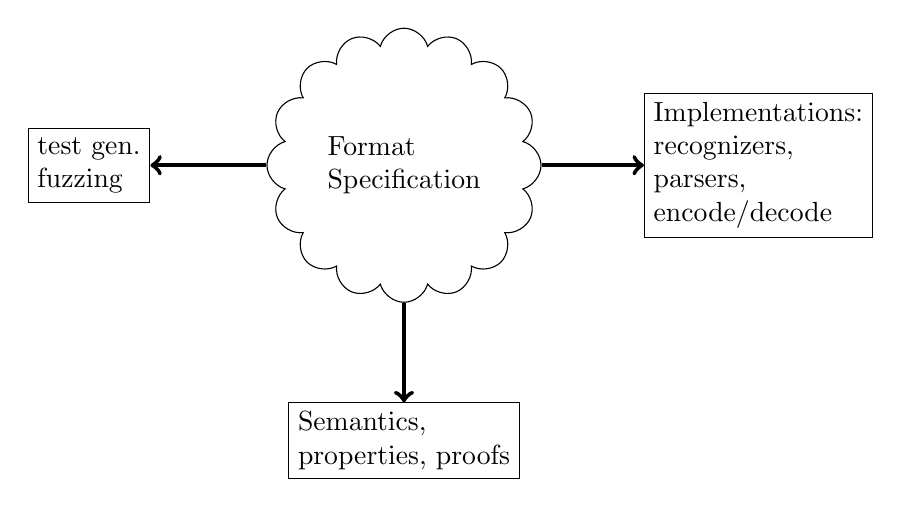
\begin{tikzpicture}[auto]

\node [cloud, draw, cloud puffs = 16, align=left] (SPEC) at (0,0) {Format \\ Specification};
\node [draw,align=left](TEST) at (-4,0) {test gen. \\ fuzzing};
\node [draw,align=left] (PROP) at (0,-3.5) {Semantics, \\ properties, proofs};
\node [draw, align=left] (IMPL) at (4.5,0) {Implementations: \\ recognizers, \\ parsers, \\ encode/decode};
\draw [->, ultra thick] (SPEC) to (TEST);
\draw [->, ultra thick] (SPEC) to (PROP);
\draw [->, ultra thick] (SPEC) to (IMPL);
\end{tikzpicture}

\end{frame}


%\section{Self-describing messages}

\begin{frame}[fragile]\frametitle{Self-describing messages}

Message formats commonly have self-describing aspects such as

\begin{itemize}

\item [$\blacktriangleright$] \gemph{length} fields, which represent
  sizes for other parts of the message, e.g., a list of elements,
  along with field telling how many elements are in the list.

\item [$\blacktriangleright$] \gemph{unions}, which allow multiple
  versions of a format to exist in a single format, e.g.  \textit{If
    field A is less than 14 then the message has 10 fields, else it
    has 15}

\end{itemize}

In general, \gemph{the deeper you go the more you know} and we need to
do a good job of modelling that accumulation of information while
recognizing/parsing.

\end{frame}

\begin{frame}\frametitle{Approaches to self-describing messages}

\begin{itemize}

\item [$\blacktriangleright$] Wouldn't it be great if some ideas from the
  vast ocean of formal language theory could be applied?

\item [$\blacktriangleright$] The self-describing aspect,
  unfortunately, hampers the use of standard lexer and parser
  technology

\item [$\blacktriangleright$] Regular languages are insufficient and
  context-free grammars also can’t capture the dependency of one field
  (or collection of fields) on another.

\end{itemize}
\end{frame}

\begin{frame}\frametitle{Approaches to self-describing messages}
\begin{itemize}

\item [$\blacktriangleright$] Context-sensitive grammars seem like a
  possibility, but they have very little tool support

\item [$\blacktriangleright$] Attribute grammars were introduced by
  Knuth for context-sensitive parsing and that technology could be
  applied.

\item [$\blacktriangleright$] Parser combinators allow hand-rolled
  parsers to be very quickly constructed, and can be adapted to
  support the accumulation and propagation of the necessary dependency
  information.

\item [$\blacktriangleright$] Also an impressive body of work using
  dependent types

\end{itemize}

We \gemph{prefer to stay on the formal language side of things} since there is
a strong connection between formatted data and the strings of formal
language theory.

\end{frame}

%% \begin{frame}\frametitle{SPLAT}

%% We need to span the gap between specifications on high level data and
%% implementations over flat strings.

%% Seek to apply ideas from Formal Language Theory to showing properties
%% of operations on high-level data.

%% \vspace*{10mm}

%% \gemph{\konst{SPLAT} = Semantic Properties over Language and Automata Theory}

%% \end{frame}

%% \begin{frame}[fragile]\frametitle{SPLAT the early days}

%% Initial version of \konst{SPLAT} was based on a HOL4 theory of regexps and regexp
%% compilation developed with Scott Owens.

%% \begin{itemize}[<+->]
%% \item [$\blacktriangleright$] Regard a message as a concatenation of \emph{fields}
%% \item [$\blacktriangleright$] Each field has an interval spec of the form $\mathit{lo} \leq \mathit{field} \leq \mathit{hi}$
%% \item [$\blacktriangleright$] An interval spec can be translated to a regexp which is a
%%   predicate on the binary representation of the field.
%% \item The concatenation of regexps for the message fields gives a big regexp for the message.
%% \item [$\blacktriangleright$] Filter is obtained by compiling (deductively) regexp to DFA.
%% \end{itemize}

%% \end{frame}


\begin{frame}[fragile]\frametitle{Contiguity Types}

The notion is that message processing consists of

\begin{itemize}
\item [$\blacktriangleright$] accumulating field information
\item [$\blacktriangleright$] computing values from that information when needed
\end{itemize}

In particular, we need

\begin{itemize}
\item [$\blacktriangleright$] Arithmetic expressions for computing length fields
\item [$\blacktriangleright$] Boolean expressions for computing decisions in unions
\end{itemize}

\end{frame}

\begin{frame}[fragile]\frametitle{Contiguity types: syntax}

The syntax of contiguity types is very similar to a standard
collection of base types closed under formation of records, arrays,
and unions.

\[
\begin{array}{rcl}
 \mathit{base} & = & \konst{bool} \mid \konst{char} \mid \konst{u8} \mid \cdots \mid \konst{u64}  \mid \konst{i16} \mid \cdots \mid \konst{i64} \mid \konst{float} \mid \konst{double} \\
 \tau & = & \mathit{base} \\
      & \mid & \konst{Recd}\; (f_1 : \tau_1) \ldots (f_n : \tau_n) \\
      & \mid & \konst{Array}\; \tau \; \mathit{exp} \\
      & \mid & \konst{Alt}\; \mathit{bexp}\; \tau_1 \; \tau_2 \qquad (\text{written}\ \konst{if}\;\mathit{bexp}\;\konst{then}\;\tau_1\;\konst{else}\; \tau_2)
\end{array}
\]

\end{frame}

\begin{frame}[fragile]\frametitle{Contiguity types: examples}

\begin{tabular}{ll}
Simple record &
\fbox{
\begin{tabular}{rcl}
  \{A & : & char \\
  B & : & i32 \\
  C & : & u32 [1024]\}
\end{tabular}
}
\\ \\

Array &
\fbox{
\begin{tabular}{rcl}
  \{len & : & u16 \\
   A   & : & i32 [\gemph{len}]\}
\end{tabular}
}
\\ \\

Array &
\fbox{
\begin{tabular}{rcl}
  \{Dims & : & \{rows :  u16 \\
         & &   {~} cols : u16\} \\
 Image & : & i32 [\gemph{Dims.rows * Dims.cols}]\}
\end{tabular}
}
\end{tabular}

\end{frame}

\begin{frame}[fragile]\frametitle{Contiguity types: examples}

Alt

\fbox{
\begin{tabular}{lcl}
  \{relno & : & u32 \\
  \phantom{\{} B & : & i32 \\
\phantom{\{} C & : &
  \konst{if}\;\gemph{relno \textless 14} \\
    & & {~~} \konst{then}\; \{D : u32 [\gemph{B}]\}) \\
    & & {~~} \konst{else}\; \{P : bool, Q : i64 [\gemph{B}]\}\}
\end{tabular}
}

\end{frame}

\begin{frame}[fragile]\frametitle{Semantics}

The semantics of contiguity types is in terms of formal languages:

\[
% \begin{array}{l}
\LangTheta{\tau} =
\mathtt{case}\; \tau\
% \hspace*{3mm}
 \left\{
 \begin{array}{l}
 \mathit{base} \Rightarrow \set{s \mid \konst{len}(s) = \konst{width}(base)} \\
 \konst{Recd}\; (f_1 : \tau_1) \ldots (f_n : \tau_n)
      \Rightarrow \LangTheta{\tau_1} \cdot \ldots \cdot \LangTheta{\tau_n}
\\
 \konst{Array}\; \tau \; \mathit{exp} \Rightarrow  \\
  \hspace*{5mm}
 \left\{
 \begin{array}{ll}
    \LangTheta{\tau}^{\konst{evalExp}\;\theta\;\mathit{exp}} &
       \mathrm{if}\; \konst{evalExp}\;\theta\;\mathit{exp}\;\Downarrow \\
    \emptyset & \text{if evaluation fails}
 \end{array}
 \right.
\\
 \konst{Alt}\; \mathit{bexp}\;\tau_1\; \tau_2 \Rightarrow \\
  \hspace*{5mm}
 \left\{
 \begin{array}{ll}
    \LangTheta{\tau_1} & \mathrm{if}\ \konst{evalBexp}\;\theta\;\mathit{bexp} = \konst{true} \\
    \LangTheta{\tau_2} & \mathrm{if}\ \konst{evalBexp}\;\theta\;\mathit{bexp} = \konst{false} \\
    \emptyset          & \text{if evaluation fails}
 \end{array}
 \right.
 \\
\end{array}
 \right.
%\end{array}
\]

\end{frame}

\begin{frame}[fragile]\frametitle{Semantics}

In words:

\begin{itemize}
\item [$\blacktriangleright$] Each base type has a width and the meaning of a base type is the
  set of all strings of the given width.

\item [$\blacktriangleright$] A record translates to the language concatenation of the translations of its fields.

\item [$\blacktriangleright$] An array $\konst{Array}\;\tau\; \mathit{exp}$ is the $n$-ary
  concatenation of the language of $\tau$, where $n$ is the value of
  $\mathit{exp}$.

\item [$\blacktriangleright$] An $\konst{Alt}\; \mathit{bexp} \;
  \tau_1 \; \tau_2$ maps to the translation of $\tau_1$ if
  $\mathit{bexp}$ evaluates to \konst{true}, and to the translation of
  $\tau_2$ if $\mathit{bexp}$ evaluates to \konst{false}

\item [$\blacktriangleright$] If any expression or boolean expression
  evaulation fails, then the empty language $\emptyset$ is the result.

\end{itemize}

\end{frame}

\begin{frame}\frametitle{Expressions}

Expressions and boolean expressions are conventional, except that we
use \gemph{L-values} instead of variables.

\[
\begin{array}{rcl}
\mathit{lval} & = & \mathit{varname} \mid
                    \mathit{lval} \, [ \mathit{exp} ] \mid
                    \mathit{lval} . \mathit{fieldname} \\
%  & & \\
\mathit{exp} & = & \konst{Loc}\; \mathit{lval}
              \mid \konst{nLit}\; \konst{nat}
              \mid \mathit{constname}
              \mid \mathit{exp} + \mathit{exp}
              \mid \mathit{exp} * \mathit{exp} \\
%  & & \\
\mathit{bexp} & = & \konst{bLoc}\; \mathit{lval}
              \mid  \konst{bLit}\; \konst{bool}
              \mid  \neg \mathit{bexp} \\
& \mid &  \mathit{bexp} \land \mathit{bexp}
              \mid  \mathit{exp} = \mathit{exp}
              \mid  \mathit{exp} < \mathit{exp}
\end{array}
\]

\textbf{Remark} Using L-values instead of variables made a big difference.

\end{frame}

\begin{frame}\frametitle{Matching algorithm}

  The main algorithm for contiguity types is a \emph{matcher}.

Function \textbf{match} takes a contig type and a string and, if
successful, returns an assignment $\theta$ of slices of the string to
elements of the type.

\begin{theorem}[Soundness]
  \[
 \vdash \konst{match}\; \mathit{contig}\; \mathit{string} = \konst{Some}(\theta) \imp
   \mathit{string} \in \LangTheta{\mathit{contig}}
\]
\end{theorem}

\textbf{match} has the flavor of a \gemph{parser generator}: it takes a
specification of the language to be parsed and returns an implementation

\end{frame}


\begin{frame}[fragile]\frametitle{Matching algorithm}

\begin{itemize}

\item [$\blacktriangleright$] Operates in \emph{worklist} style

\item [$\blacktriangleright$] Flattens contig-type down until a base type is exposed

\item [$\blacktriangleright$] At base type, the corresponding location
  is generated and added to context $\theta$

\item [$\blacktriangleright$] Easy to instrument a version in order to produce parse trees

\item [$\blacktriangleright$] \gemph{Incredibly simple implementation} (approx 200 lines of SML)

\item [$\blacktriangleright$] HOL4 formalization available on GitHub. (See paper for URL).

\end{itemize}

\end{frame}

\begin{frame}\frametitle{Assertions}

An unanticipated gift: \gemph{in-message assertions can be expressed.}

\[
\begin{array}{l}
\konst{Assert}\;\mathit{bexp}  =
\konst{if}\; \mathit{bexp}\; \konst{then}\; \konst{SKIP} \;\konst{else}\;\konst{Void} \\
\konst{SKIP} = \konst{Recd} [\, ] \\
\konst{Void} = \text{nullary constructor, denoting } \emptyset
\end{array}
\]

\begin{description}
\item [Declaratively] Evaluate the boolean expression in the current context;
  if it is true then $\varepsilon$ else $\emptyset$,

\item [Operationally] Check the property; if it is true, continue on
  without consuming input; if false, fail.
\end{description}


We use assertions extensively in our application work to enforce
well-formedness properties on messages.

\end{frame}

\begin{frame}[fragile]\frametitle{Bounded $A^n B^n C^n$}

\[
\begin{array}{l}
  \mathit{charA} = \{ch : char, \,isA : \konst{Assert} (ch = 65)\} \\
  \mathit{charB} = \{ch : char, \,isB : \konst{Assert} (ch = 66)\} \\
  \mathit{charC} = \{ch : char, \,isC : \konst{Assert} (ch = 67)\} \\
\\
\begin{array}{l}
\mathit{mesg} = \{\mathit{len} : u16 \\
\phantom{\mathit{mesg} = \{} A : \mathit{charA}\, [len] \\
\phantom{\mathit{mesg} = \{} B : \mathit{charB}\, [len] \\
\phantom{\mathit{mesg} = \{} C : \mathit{charC}\, [len] \\
  \}
\end{array}
\end{array}
\]
%
In fact:
%
\[ \LangTheta{\konst{mesg}} = u \cdot A^{\konst{toN}(u)} \cdot
B^{\konst{toN}(u)} \cdot C^{\konst{toN}(u)} \]


\end{frame}

\begin{frame}\frametitle{Extension: Lists}

In order to support unbounded data, we have added lists. The type
$\konst{List}\;\tau$ is represented by the following recursive record:
%
\[
 \konst{List}\;\tau =
   \left\{
     \begin{array}{lcl}
       \mathit{tag} & : & \konst{u8} \\
        \mathit{check} & : &
         \konst{Assert}\ \mathit{tag} = \konst{NilTag} \lor \mathit{tag} = \konst{ConsTag} \\
       \mathit{test} & : &
       \begin{array}[t] {l}
         \konst{if}\; \konst{tag} = \konst{NilTag}\; \konst{then}\; \varepsilon \\
          \konst{else}\; \{ \mathit{hd} : \tau, \ \mathit{tl} : \konst{List}\; \tau \}
       \end{array}
     \end{array}
   \right.
\]

This essentially implements an unrolling of the formal language identity
%
\[ \kstar{L} = \varepsilon \cup L \cdot \kstar{L} \]


\end{frame}

%% In words, a $\konst{List}\;\tau$ matches a sequence of records where
%% a single-byte tag (\konst{NilTag} or \konst{ConsTag}) is read, then tested to see
%% whether to stop parsing the list (\konst{NilTag}) or to continue on to
%% parse a $\tau$ into the \konst{hd} field and recurse in order to
%% process the remainder of the list. An incorrect value for the tag results in failure.

\section {Application: Architectural Transformations in CASE}

\begin{frame}\frametitle{System Architecture Languages}
\begin{itemize}

\item [$\blacktriangleright$] General setting: \textbf{Architectural Design Languages}

\item [$\blacktriangleright$] An ADL supports complete, highly abstract, views of a system,
  including hardware, software, (and possibly humans)

\item [$\blacktriangleright$] An architecture model should provide a high-level setting in which
  the \gemph{whole picture} of a system can be surveyed

\item [$\blacktriangleright$] Thus: a place where existing
  implementations, new design features, high-level requirements,
  implementations, and verifications can be combined.

\item [$\blacktriangleright$] Not just boxes and arrows!

\end{itemize}

\end{frame}

\begin{frame}\frametitle{CASE}
\begin{itemize}

\item [$\blacktriangleright$] In the DARPA \textbf{CASE} project we
  are developing the idea of \gemph{Security-Enhancing}
  transformations on system architecture descriptions.

\item [$\blacktriangleright$] The goal is to develop a methodology where
  \begin{enumerate}

  \item the structure of an existing (legacy) system is captured in an
    architectural model;

 \item system security is automatically analyzed and any security
   problems are addressed by applying architectural transformations

  \end{enumerate}

\item [$\blacktriangleright$] \gemph{Key aspect}: automatic synthesis of
  security-enforcing code from a formal specification
  language. Contiguity types are at the heart of the specifications
  and synthesis.

\end{itemize}

\end{frame}

\begin{frame}[fragile]\frametitle{CASE Website}

Check it out:

\begin{verbatim}
  http://loonwerks.com/projects/case.html
\end{verbatim}

\end{frame}


\begin{frame}\frametitle{Architecture Transformations}

An architecture-to-architecture map that can be applied to
\gemph{provably increase} the security of a system.

\vspace*{4mm}

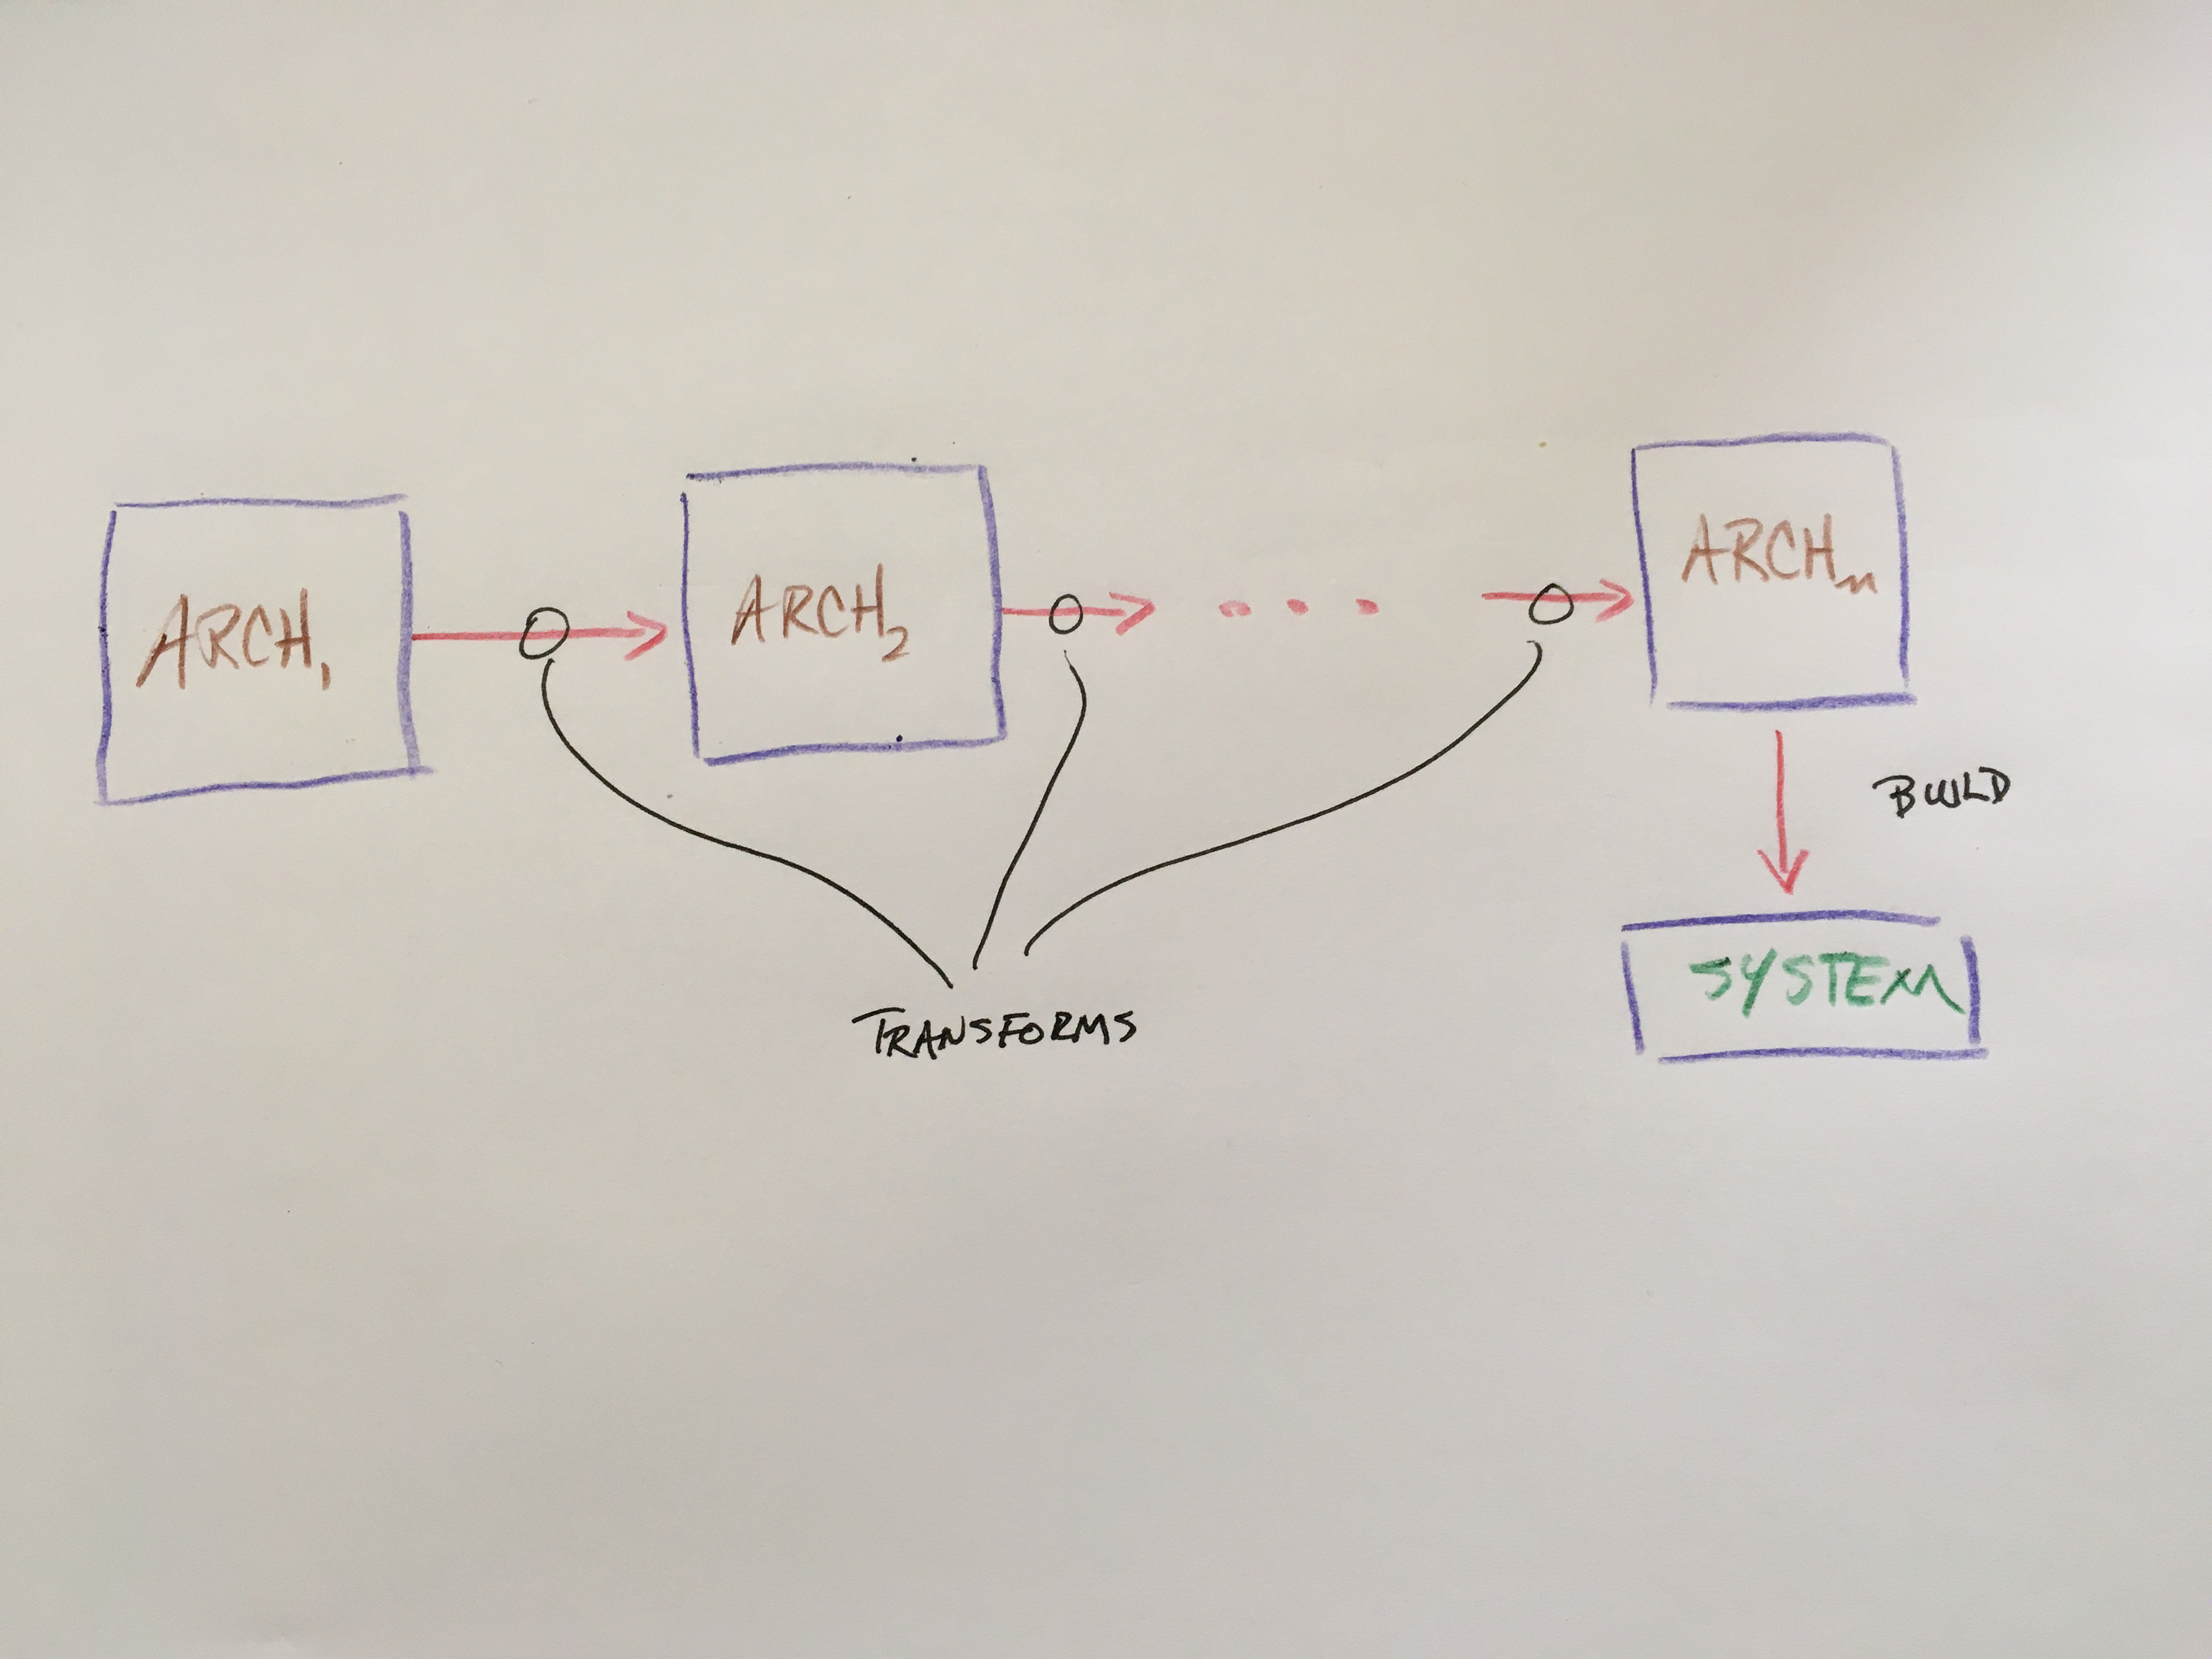
\includegraphics[width=90mm,height=50mm]{arch-trans.jpg}
\end{frame}

\begin{frame}\frametitle{Transformation: Message Filtering}

A \emph{filter} is conceptually very simple: it checks validity of its
input data according to predicate $P$.


\begin{center}
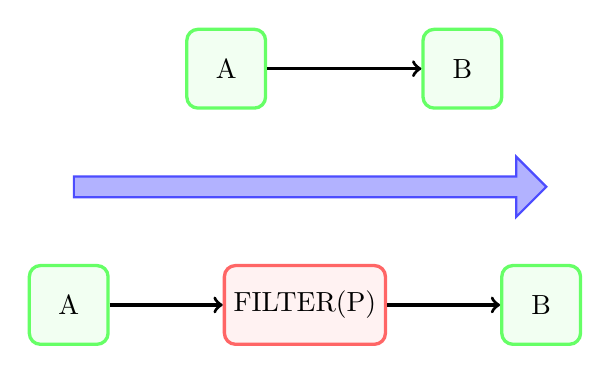
\begin{tikzpicture}[
redsquarednode/.style={rectangle, draw=red!60, fill=red!5, very thick, rounded corners, minimum size=10mm},
greensquarednode/.style={rectangle, draw=green!60, fill=green!5, very thick, rounded corners, minimum size=10mm},
fat arrow/.style={single arrow,thick,draw=blue!70,fill=blue!30,minimum height=60mm,minimum width=7mm}
]
%Nodes
\node[draw,greensquarednode] at (2,0) (SRC)    {A};
\node[draw,greensquarednode] at (5,0) (TARGET) {B};

%\node at (3.5,-1.5) [fat arrow]{};
\node at (3,-1.5) [fat arrow]{};

\node[draw,greensquarednode] at (0,-3) (SRC-1)    {A};
\node[draw,greensquarednode] at (6,-3) (TARGET-1) {B};
\node[draw,redsquarednode] at (3,-3) (FILTER) {FILTER(P)};

%Lines
\draw[->,very thick] (SRC.east) -- (TARGET.west);

\draw[->,very thick] (SRC-1.east) -- (FILTER.west);
\draw[->,very thick] (FILTER.east) -- (TARGET-1.west);
\end{tikzpicture}
\end{center}

%% \hspace*{10mm}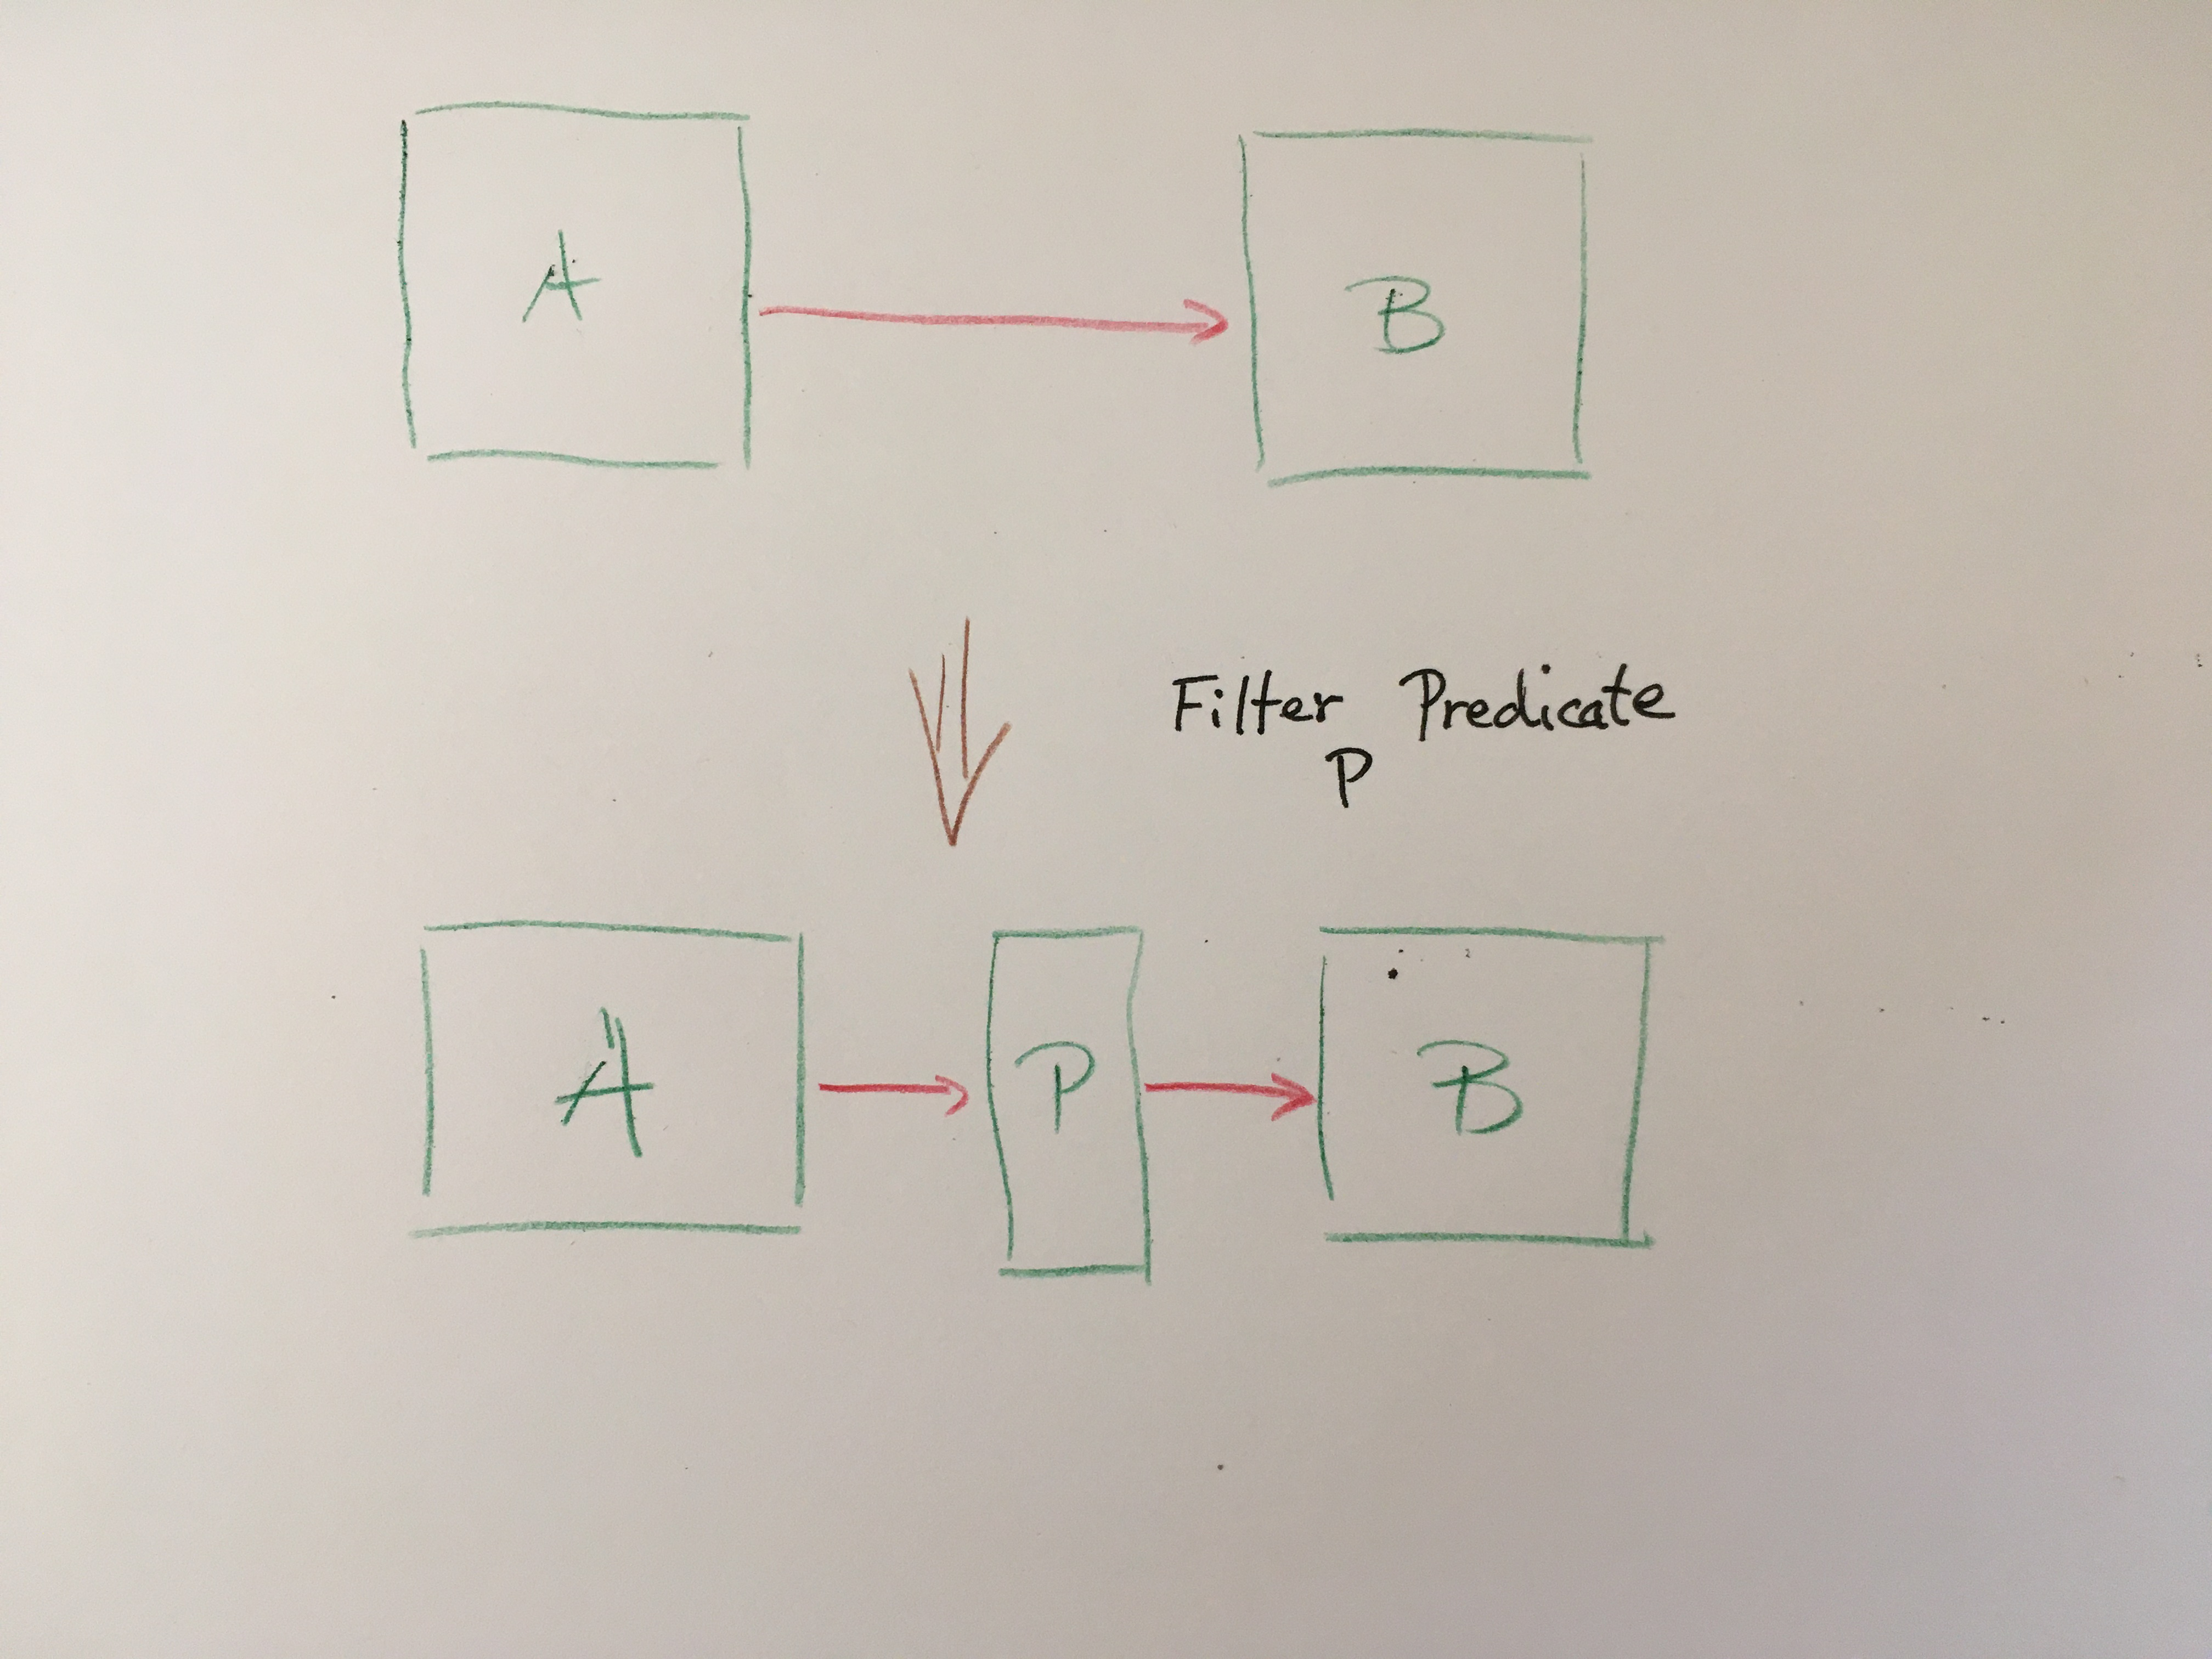
\includegraphics[width=90mm,height=50mm]{filter.jpg}

If the data is valid, then it is passed on. Otherwise it is dropped.

\end{frame}


\begin{frame}\frametitle{Transformation: Message Monitoring}

A \emph{monitor} checks to see that a relationship $\mathcal{R}$ holds
over a collection of message streams through time. If the
specification is violated, an \emph{alert} is sent out.

\begin{center}
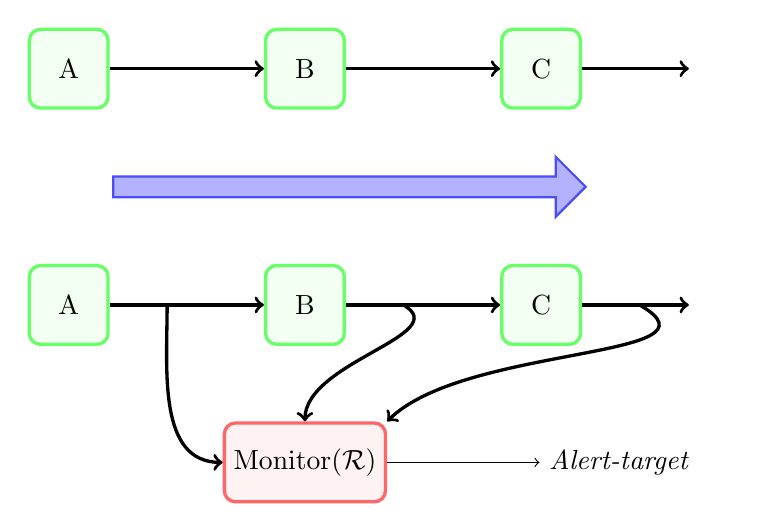
\begin{tikzpicture}[
redsquarednode/.style={rectangle, draw=red!60, fill=red!5, very thick, rounded corners, minimum size=10mm},
greensquarednode/.style={rectangle, draw=green!60, fill=green!5, very thick, rounded corners, minimum size=10mm},
fat arrow/.style={single arrow,thick,draw=blue!70,fill=blue!30,minimum height=60mm,minimum width=7mm}
]
%Nodes
\node[draw,greensquarednode] at (1,0) (A) {A};
\node[draw,greensquarednode] at (4,0) (B) {B};
\node[draw,greensquarednode] at (7,0) (C) {C};
\node at (9,0) (D) {};

\node at (4.5,-1.5) [fat arrow]{};

\node[draw,greensquarednode] at (1,-3) (A-1) {A};
\node at (2.25,-3) (joinAB) {};
\node[draw,greensquarednode] at (4,-3) (B-1) {B};
\node at (5.25,-3) (joinBC) {};
\node[draw,greensquarednode] at (7,-3) (C-1) {C};
\node at (8.25,-3) (joinCD) {};
\node at (9,-3) (D-1) {};
\node[draw,redsquarednode]   at (4,-5) (M) {Monitor($\mathcal{R}$)};
\node at (8,-5) (ALERT-TARGET) {\textit{Alert-target}};

%Lines
\draw[->,very thick] (A.east) -- (B.west);
\draw[->,very thick] (B.east) -- (C.west);
\draw[->,very thick] (C.east) -- (D.west);
\draw[->,very thick] (A-1.east) -- (B-1.west);
\draw[->,very thick] (B-1.east) -- (C-1.west);
\draw[->,very thick] (C-1.east) -- (D-1.west);

\draw[->,very thick] (2.25,-3) to [out=-90, in=180] (M);
\draw[->,very thick] (5.25,-3) to [out=-30, in=90]  (M);
\draw[->,very thick] (8.25,-3) to [out=-30, in=45]  (M.north east);
\draw[->] (M.east) -- (ALERT-TARGET);

\end{tikzpicture}
\end{center}

%% \hspace*{10mm}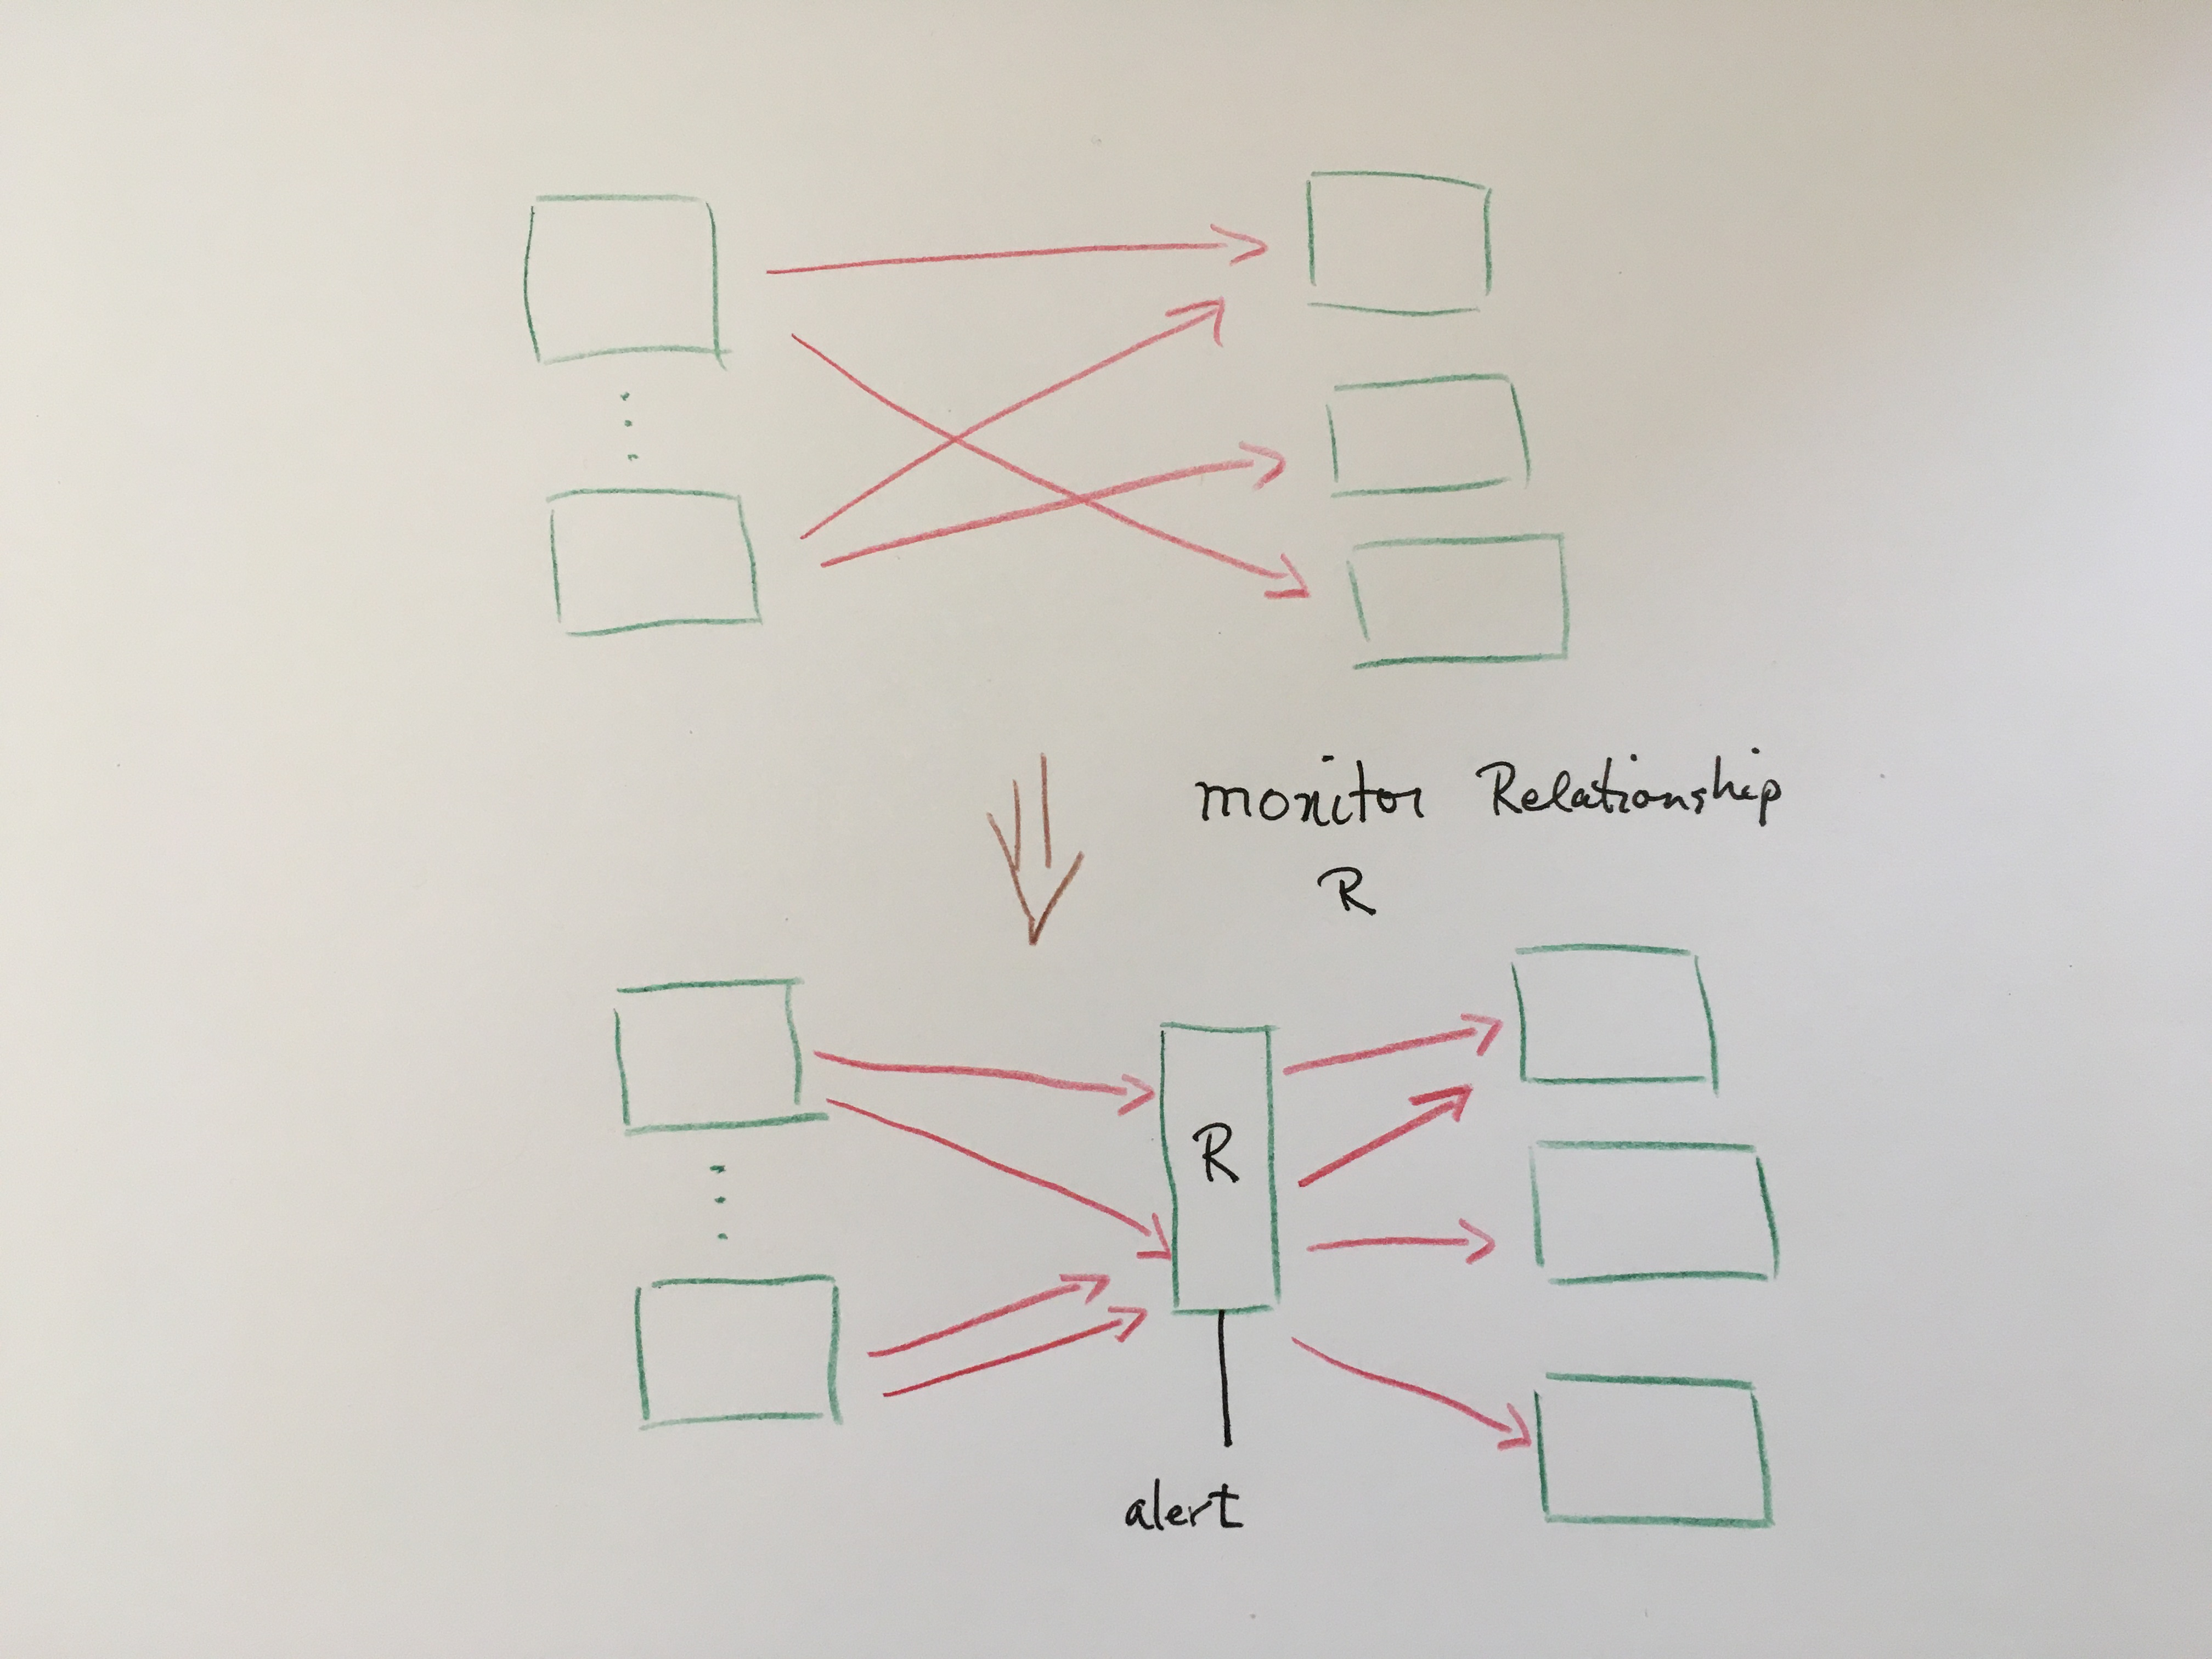
\includegraphics[width=90mm,height=40mm]{monitor.jpg}

\end{frame}

\begin{frame}\frametitle{Transformation: Isolation of `at risk' components}

An unprotected computational element can be isolated by transparently
lifting it out of its context and mediating access via seL4.

\begin{center}
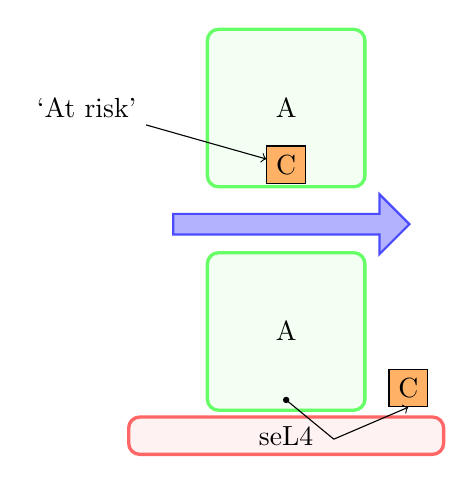
\begin{tikzpicture}[
bignode/.style =
  {rectangle,
   draw=green!60, fill=green!5,
   very thick, rounded corners,
   minimum height=20mm, minimum width = 20mm},
flatnode/.style =
  {rectangle,
   draw=red!60, fill=red!5,
   very thick, rounded corners,
   minimum width = 40mm},
fat arrow/.style={single arrow,thick,draw=blue!70,fill=blue!30,minimum height=30mm,minimum width=7mm}
]
%Nodes
\node[draw,bignode](main){A};
\node[draw,fill=orange!60] (atrisk) at ([yshift=2ex]main.south){C};
\node (comment) at ([xshift=-10ex]main.west){`At risk'};
\draw[->] (comment) -- (atrisk);
\node at ([yshift=-3ex]main.south) [fat arrow]{};
\node[draw,bignode](main-1) at ([yshift=-12ex]main.south){A};
\node[draw,fill=orange!60] (secure) at ([xshift=3.5ex,yshift=2ex]main-1.south east){C};
\node[draw,flatnode] (seL4) at ([yshift=-2ex]main-1.south){seL4};
\node[draw,fill=black,circle,scale = 0.2] (origin) at ([yshift=1ex]main-1.south){};
\node (foo) at ([yshift=-2ex,xshift=4ex]seL4.north){};
\draw (origin) -- (foo.center);
\draw[->] (foo.center) -- (secure.south);
\end{tikzpicture}
\end{center}

%\filldraw[black] (0,0) circle (2pt) node[anchor=west] {Intersection point};
%\hspace*{10mm}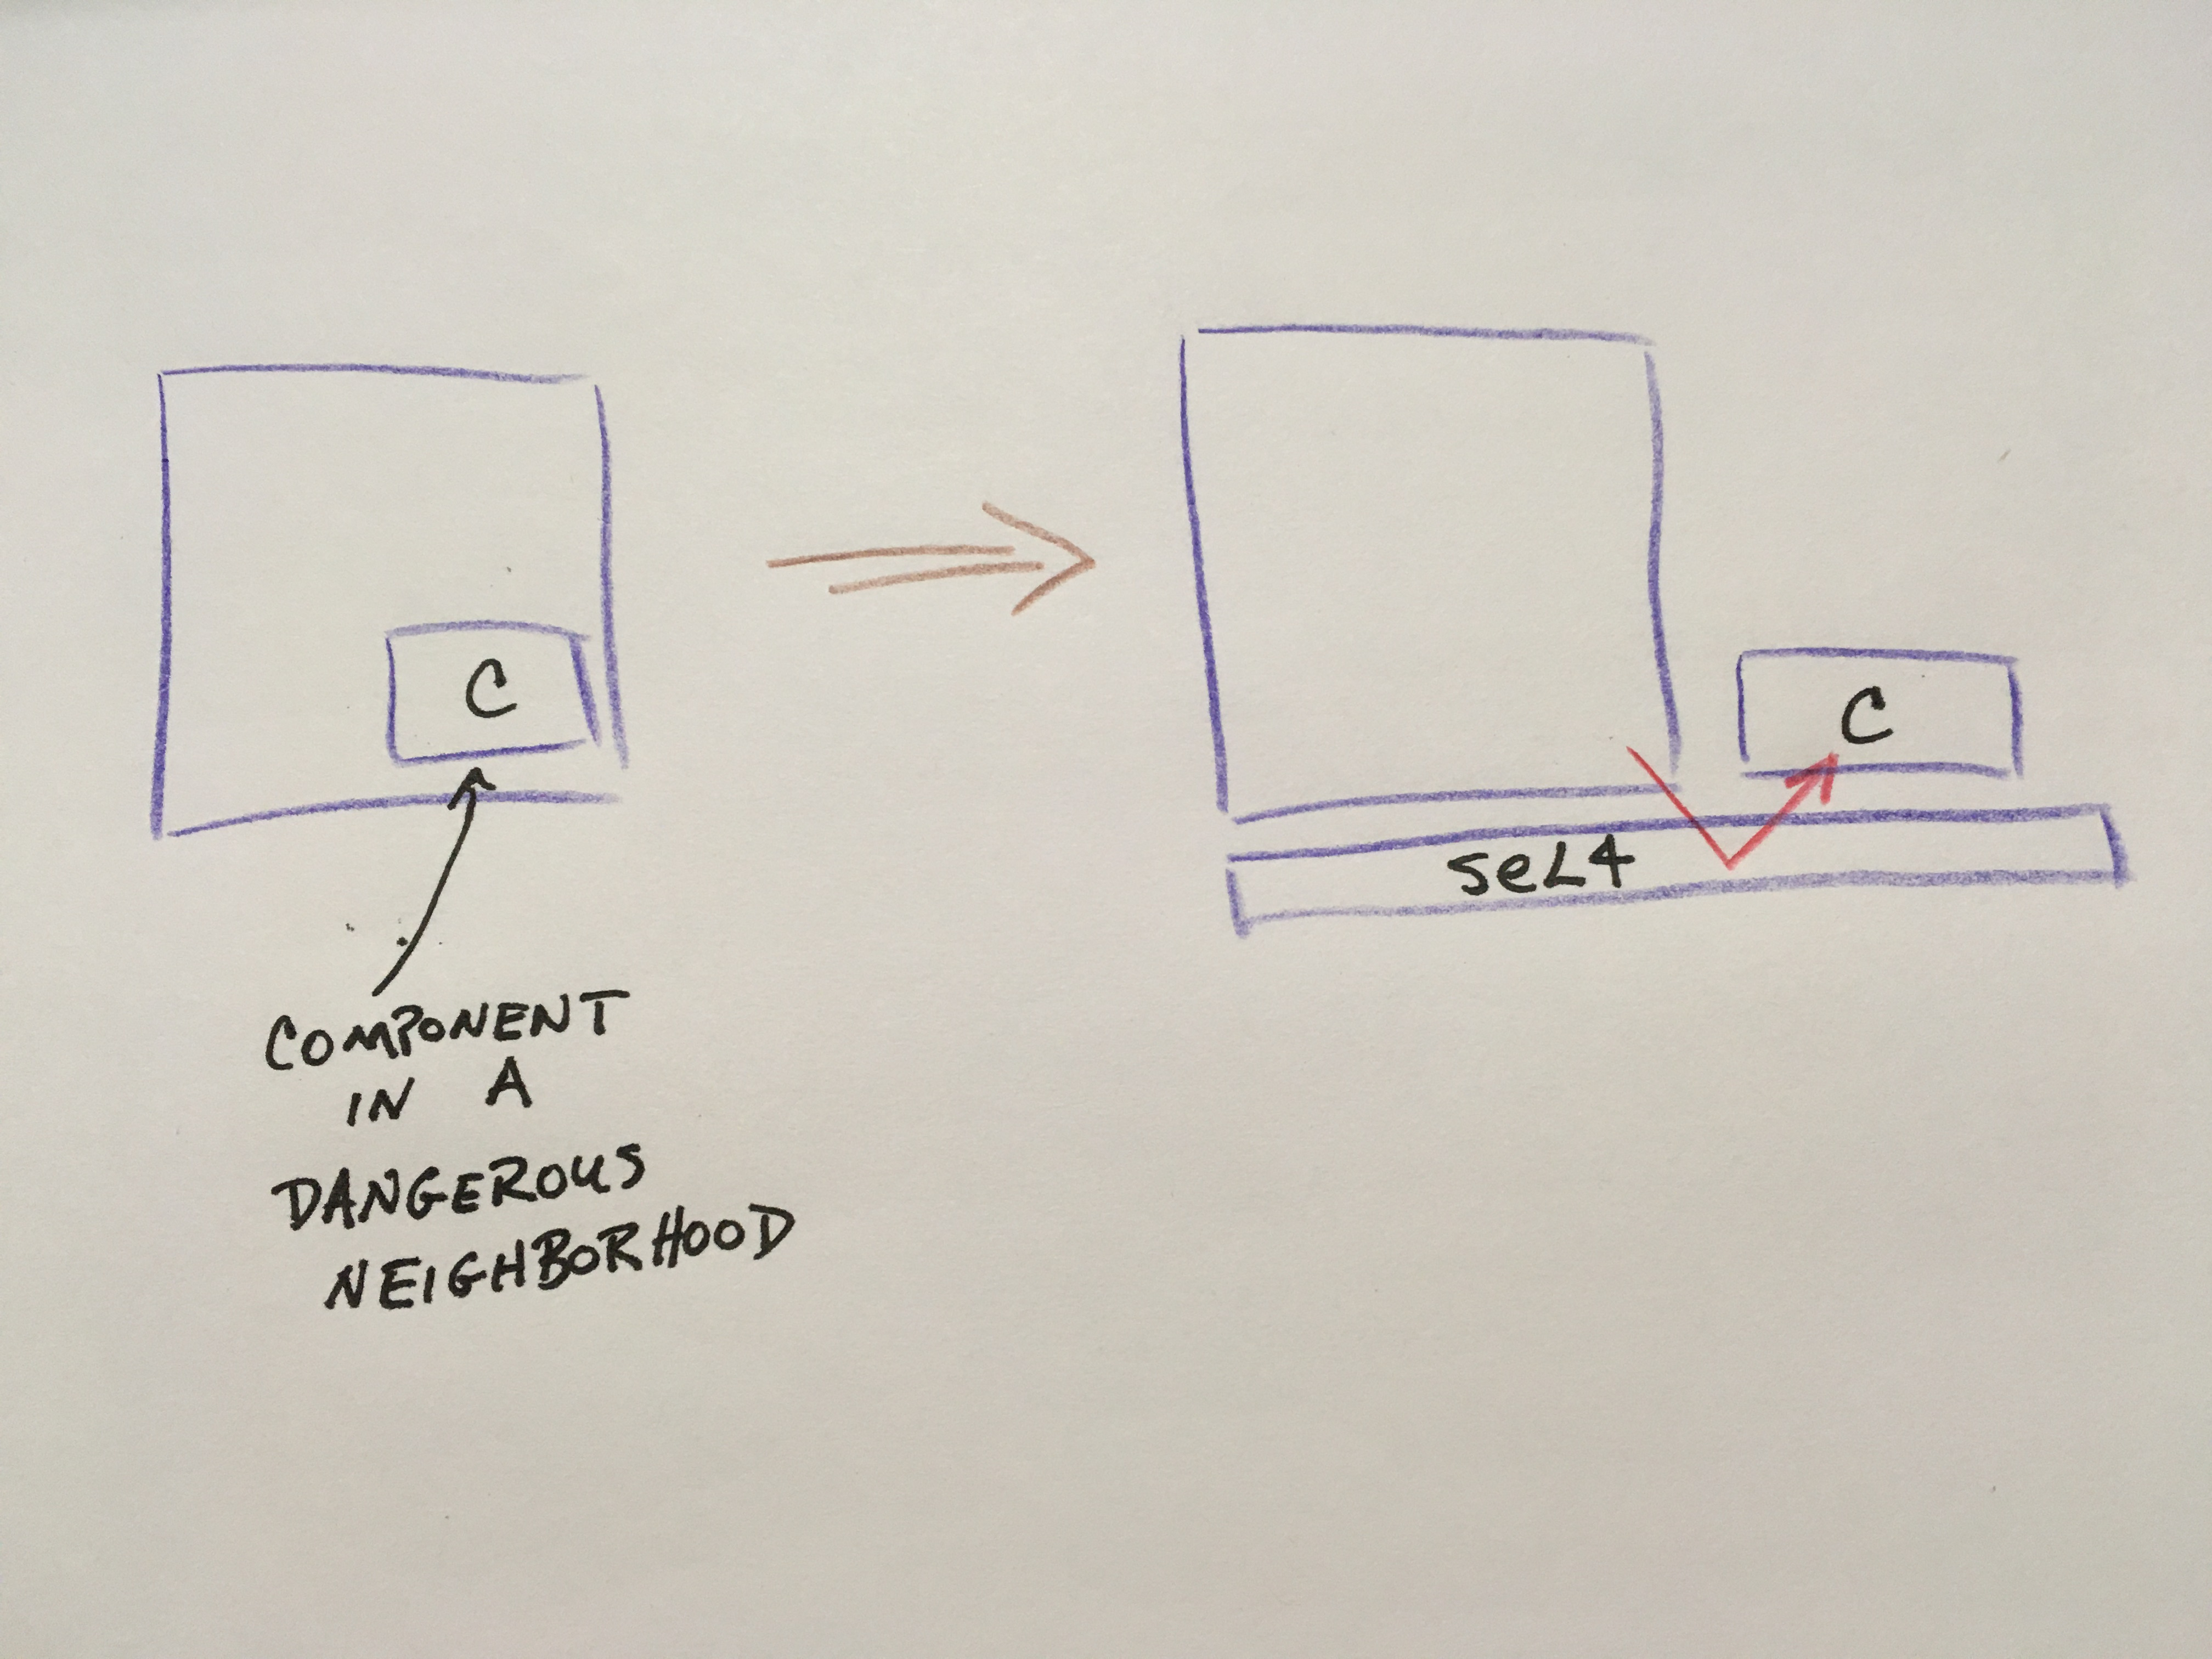
\includegraphics[width=90mm,height=40mm]{vm.jpg}

\end{frame}

\begin{frame}\frametitle{seL4 and CakeML}

Correctness of our transformations depends on formal guarantees provided by seL4 and CakeML.

\vspace*{5mm}
\hspace*{10mm}
\includegraphics[width=20mm,height=20mm]{proofcraft.png}
\hspace*{10mm}
\includegraphics[width=20mm,height=20mm]{cakeml-logo.png}

We synthesize filters and monitors to CakeML source, using Contiguity
Types to specify message formats and well-formedness conditions.


\end{frame}


\begin{frame}\frametitle{Message Format Characteristics}

The message formats we have been working with are two endpoints in a spectrum:


\begin{description}

\item [UxAS] byte oriented, complex messages, deeply nested use of
  variable-length arrays and unions

\item [ADS-B] bit oriented, no dependencies between fields, embedded real-time systems.

\end{description}

So far, contiguity types have been adequate to the demands of the project.

\end{frame}


\begin{frame}\frametitle{Current and  Future Work}

\begin{itemize}

\item [$\blacktriangleright$] Symbolic evaluation of a contig-type in
  the semantics to automatically \emph{pull out} properties

\item [$\blacktriangleright$] Tackle completeness proof

\item [$\blacktriangleright$] Compiling contig-types into fast copy-free implementations

\item [$\blacktriangleright$] Connect with recent work on formal proofs of space usage in CakeML

\item [$\blacktriangleright$] Comparison with dependent type approach

\item [$\blacktriangleright$] Understand the relationship with conventional parser technology

\item [$\blacktriangleright$] Wonderful pedagogical example (IMHO).

\end{itemize}

\end{frame}

\begin{frame}[fragile]\frametitle{End}
\end{frame}



\begin{frame}[fragile]\frametitle{Wellformed GPS}

{\small
\begin{verbatim}
 AltitudeType = AGL | MSL

 Location3D = {
  Latitude  : f64
  Longitude : f64
  Altitude  : f32
  AltitudeType : AltitudeType
  Good-Location-Check :
    -90.0 <= Latitude <= 90.0 and
   -180.0 <= Longitude <= 180.0 and
      0.0 <= Altitude <= 15000.0
  }
\end{verbatim}
}

\end{frame}

\begin{frame}[fragile]\frametitle{Wellformed GPS predicate}

Symbolic simulation of $\LangTheta{\konst{Location3D}}$ yielding

\[
\begin{array}{l}
 s \in \LangTheta{\konst{Location3D}} \iff \\
\quad   \exists s_1 s_2 s_3 s_4. \\
\qquad      s = s_1 \bullet s_2 \bullet s_3 \bullet s_4 \ \land \\
\qquad    -90.0 \leq \konst{doubleVal}(s_1) \leq 90.0 \ \land \\
\qquad   -180.0 \leq \konst{doubleVal}(s_2) \leq 180.0 \ \land \\
\qquad      0.0 \leq \konst{floatVal}(s_3)  \leq 15000.0 \ \land \\
\qquad        0 \leq \konst{natVal}(s_4) \leq 1
\end{array}
\]
%
\noindent where
%
\[
\begin{array}{ll}
 \konst{doubleVal} & : \konst{string} \to \konst{double} \\
 \konst{floatVal}  & : \konst{string} \to \konst{float}  \\
 \konst{natVal}    & : \konst{string} \to \konst{nat}  \\
\end{array}
\]

\end{frame}

\end{document}
